% !TeX spellcheck = en_US
\chapter{Implementation and Validation}%

The first step of the validation involves constructing a basic model that captures the kinematics and dynamics of an industrial robot. To test the method in a simple case, the first tests are performed on a 6-DoF model with one redundant DoF. After validation on this simple model, additional redundant DoF are introduced. 

Once the basic mathematical model is established, various optimization algorithms are implemented to determine the optimal values for each parameter associated with the redundant DoF. These methods and optimization algorithms can consider the industrial robot's specific objectives and constraints, like energy consumption or joint accelerations. 

After that, the goal is to incorporate this method with a selected CAM software to be tested in more complex scenarios.

Further validation processes entails conducting real-world tests and simulations to evaluate optimized parameter performance and verify the effectiveness of the proposed methodology.
\section{Simple Implementation}%
\subsection{Modeling a 6-DoF robot}
In order to test the proposed method, a simple articulated 6-DoF industrial robot is used as a model. A visualization of that robot is given in figure \ref{robotprog}. The Denavit-Hartenberg (DH) parameters for this robot can be found in Table \ref{DH}.


\begin{table}[H]
	\centering
	\begin{tabular}{||l|l|r||}
		  & Values \\
		\hline
		\hline
		\hline
		a	& [180, 600, 120, 0, 0, 0] \\
		alpha	&  [90, 0, 90, 90, 90, 0] \\
		d	& [400, 0, 0, 620, 0, 115]\\
		
		\hline
		\hline
	\end{tabular}
	
	\caption{DH-parameters for the modeled robot}
	\label{DH}
\end{table}

These parameters describe the geometry and kinematics of a robotic arm. They are used to define the relationship between adjacent links in a robot's kinematic chain. The DH parameters include values such as link lengths, link twists and link offsets. In this model, "a" represents the link lengths between adjacent joints, "alpha" represents the link twists or rotations around the z-axis between adjacent joints and "d" represents the link offsets or distances along the z-axis between adjacent joints. 

The arrows represent the coordinate axis of the TCP. For simplicity, the TCP is equal to the end point of the last joint. The X-axis is shown in red while the green and blue are the Y-axis and Z-axis respectively. The first link is shown in green and originates at the point X=0 Y=0 Z=0.

 \begin{figure}[H]
	\centerline{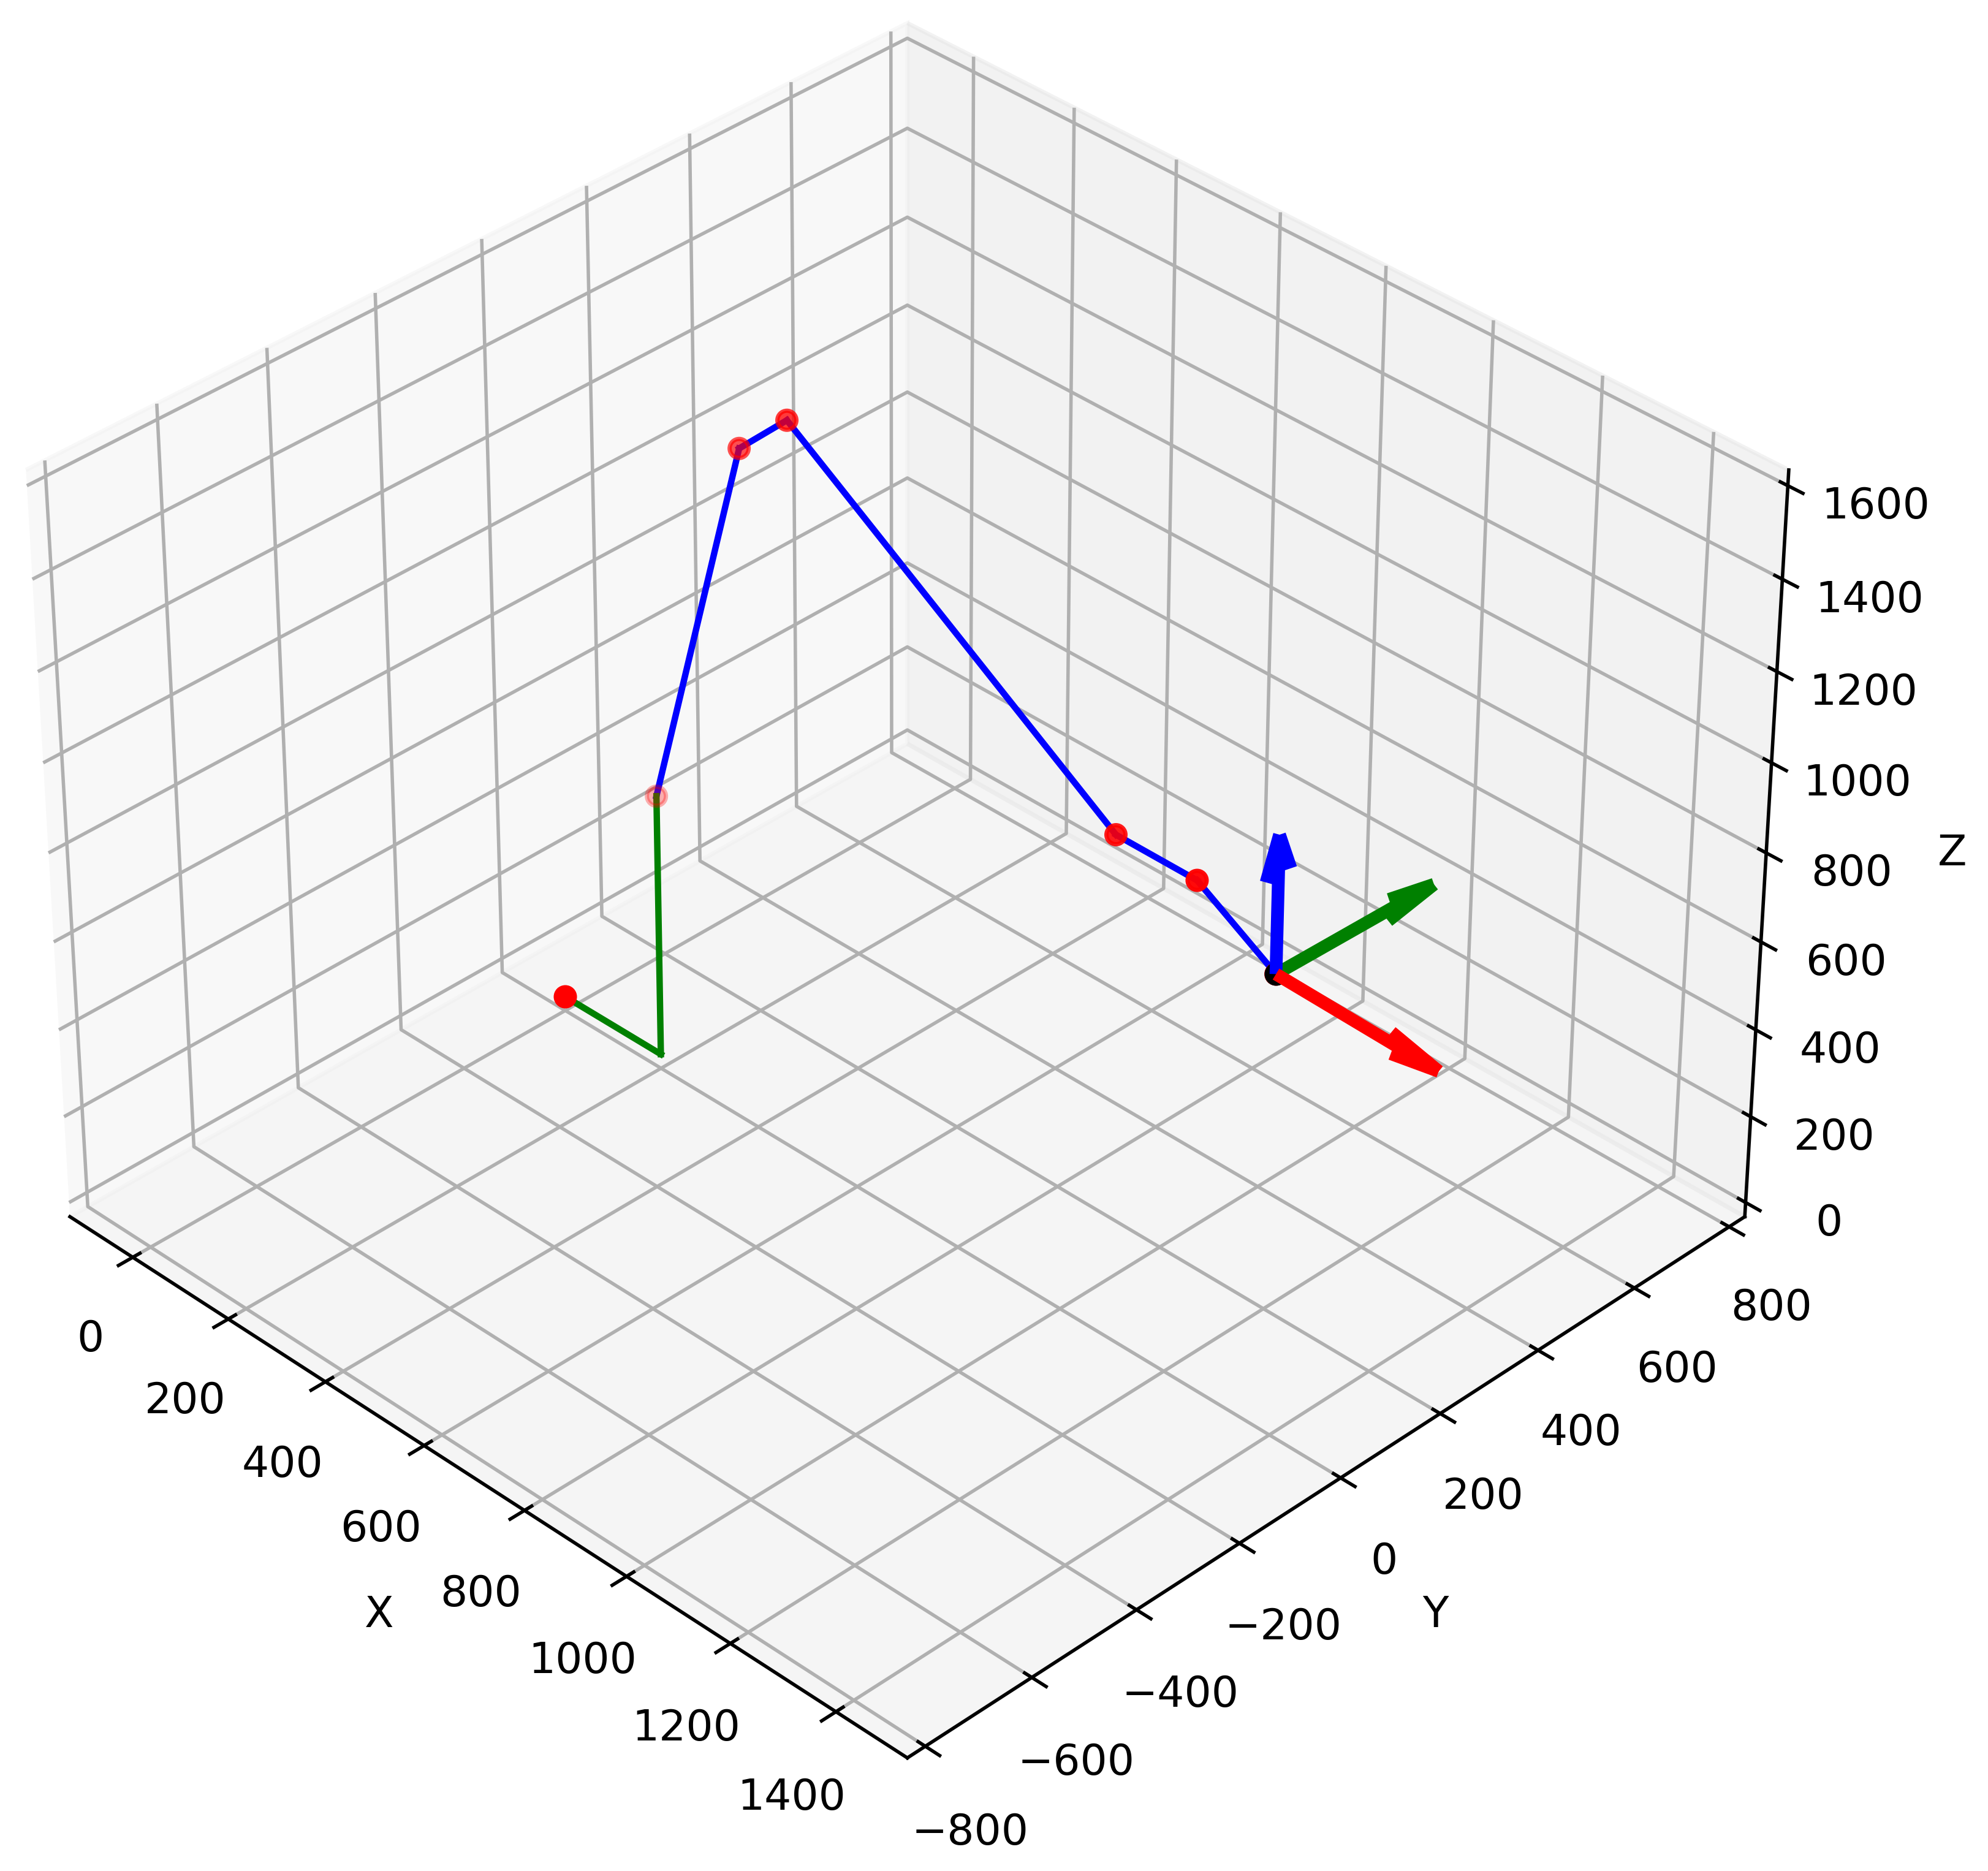
\includegraphics[width=0.7\textwidth]{figures/robotprog.png}}
	\caption{Visualization of the modeled robot}
	\label{robotprog}
\end{figure}

\subsection{Modeling a basic Toolpath}
Before the process parameters can be analyzed, a toolpath needs to be defined for the TCP to follow. In this particular case, three possible options are presented. Each toolpath consists of 2500 coordinates. It is important to note that in these cases, the redundant DoF is the rotation around the C-Axis. This means that  this rotation will be adjusted to identify the most optimal value for the desired outcome.


 \begin{figure}[H]
	\centerline{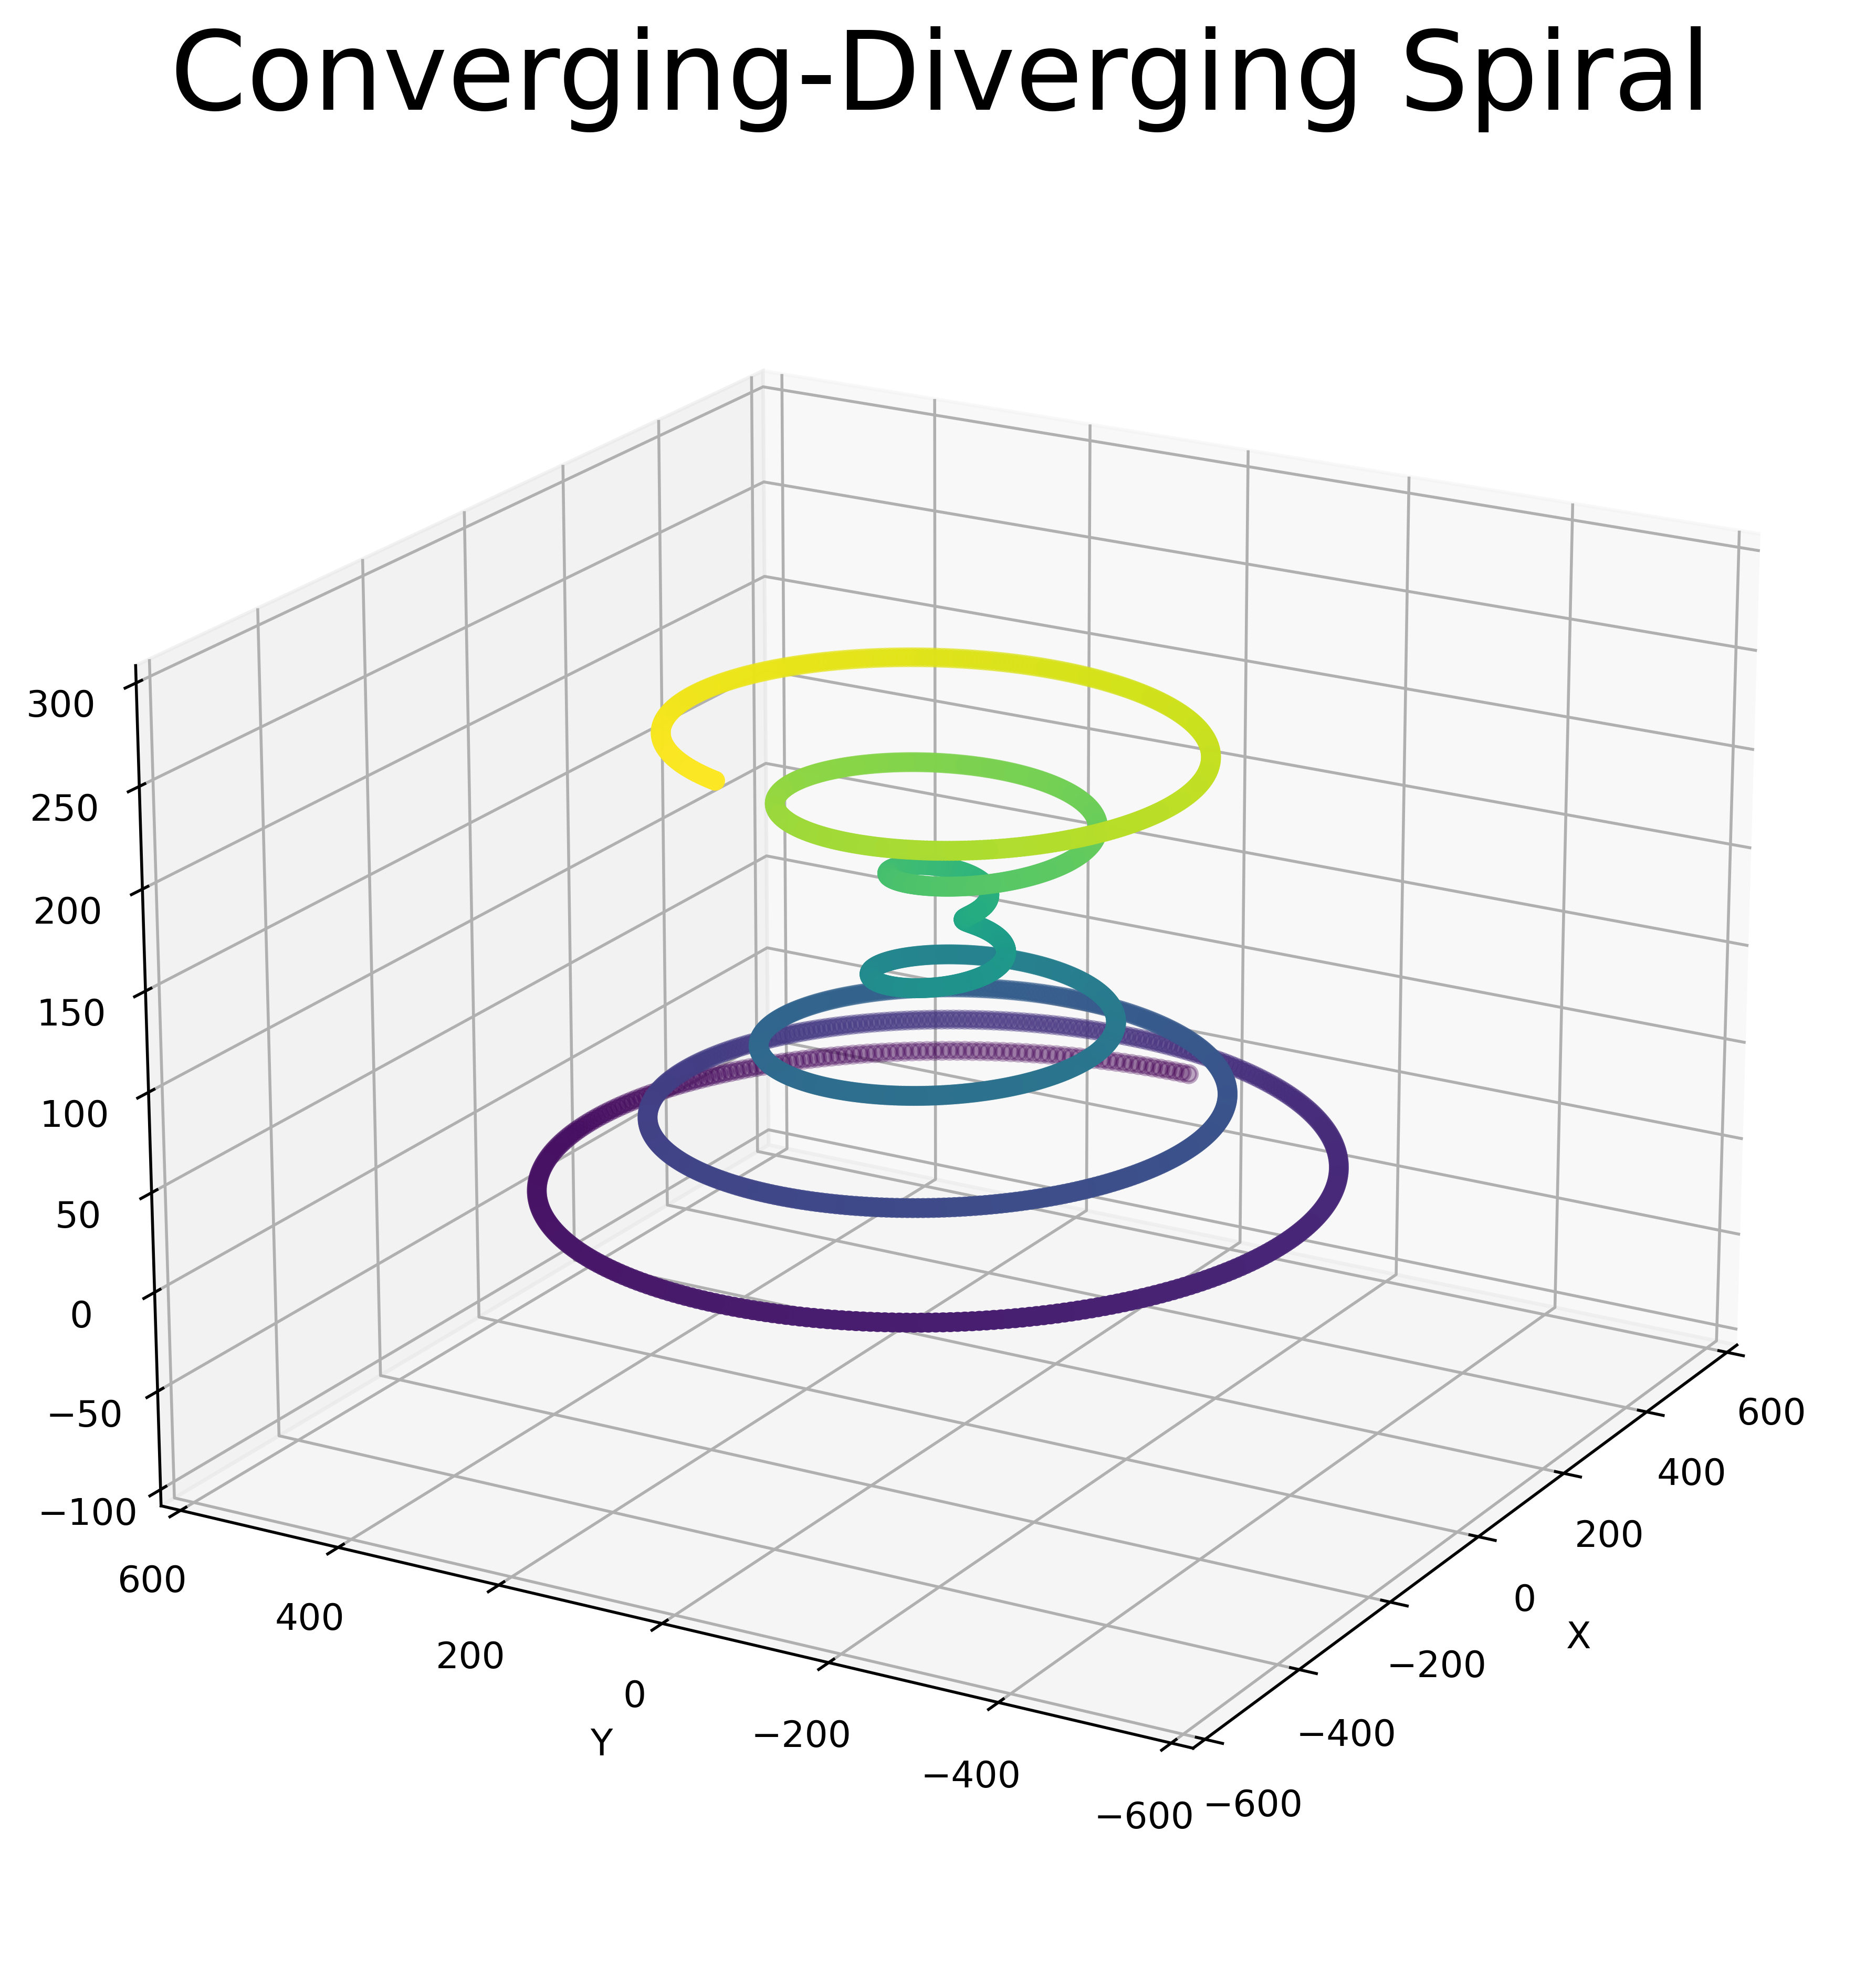
\includegraphics[width=0.5\textwidth]{figures/path1.png}}
	\caption{xxx}
	\label{xxx}
\end{figure}
\begin{figure}[H]
	\centerline{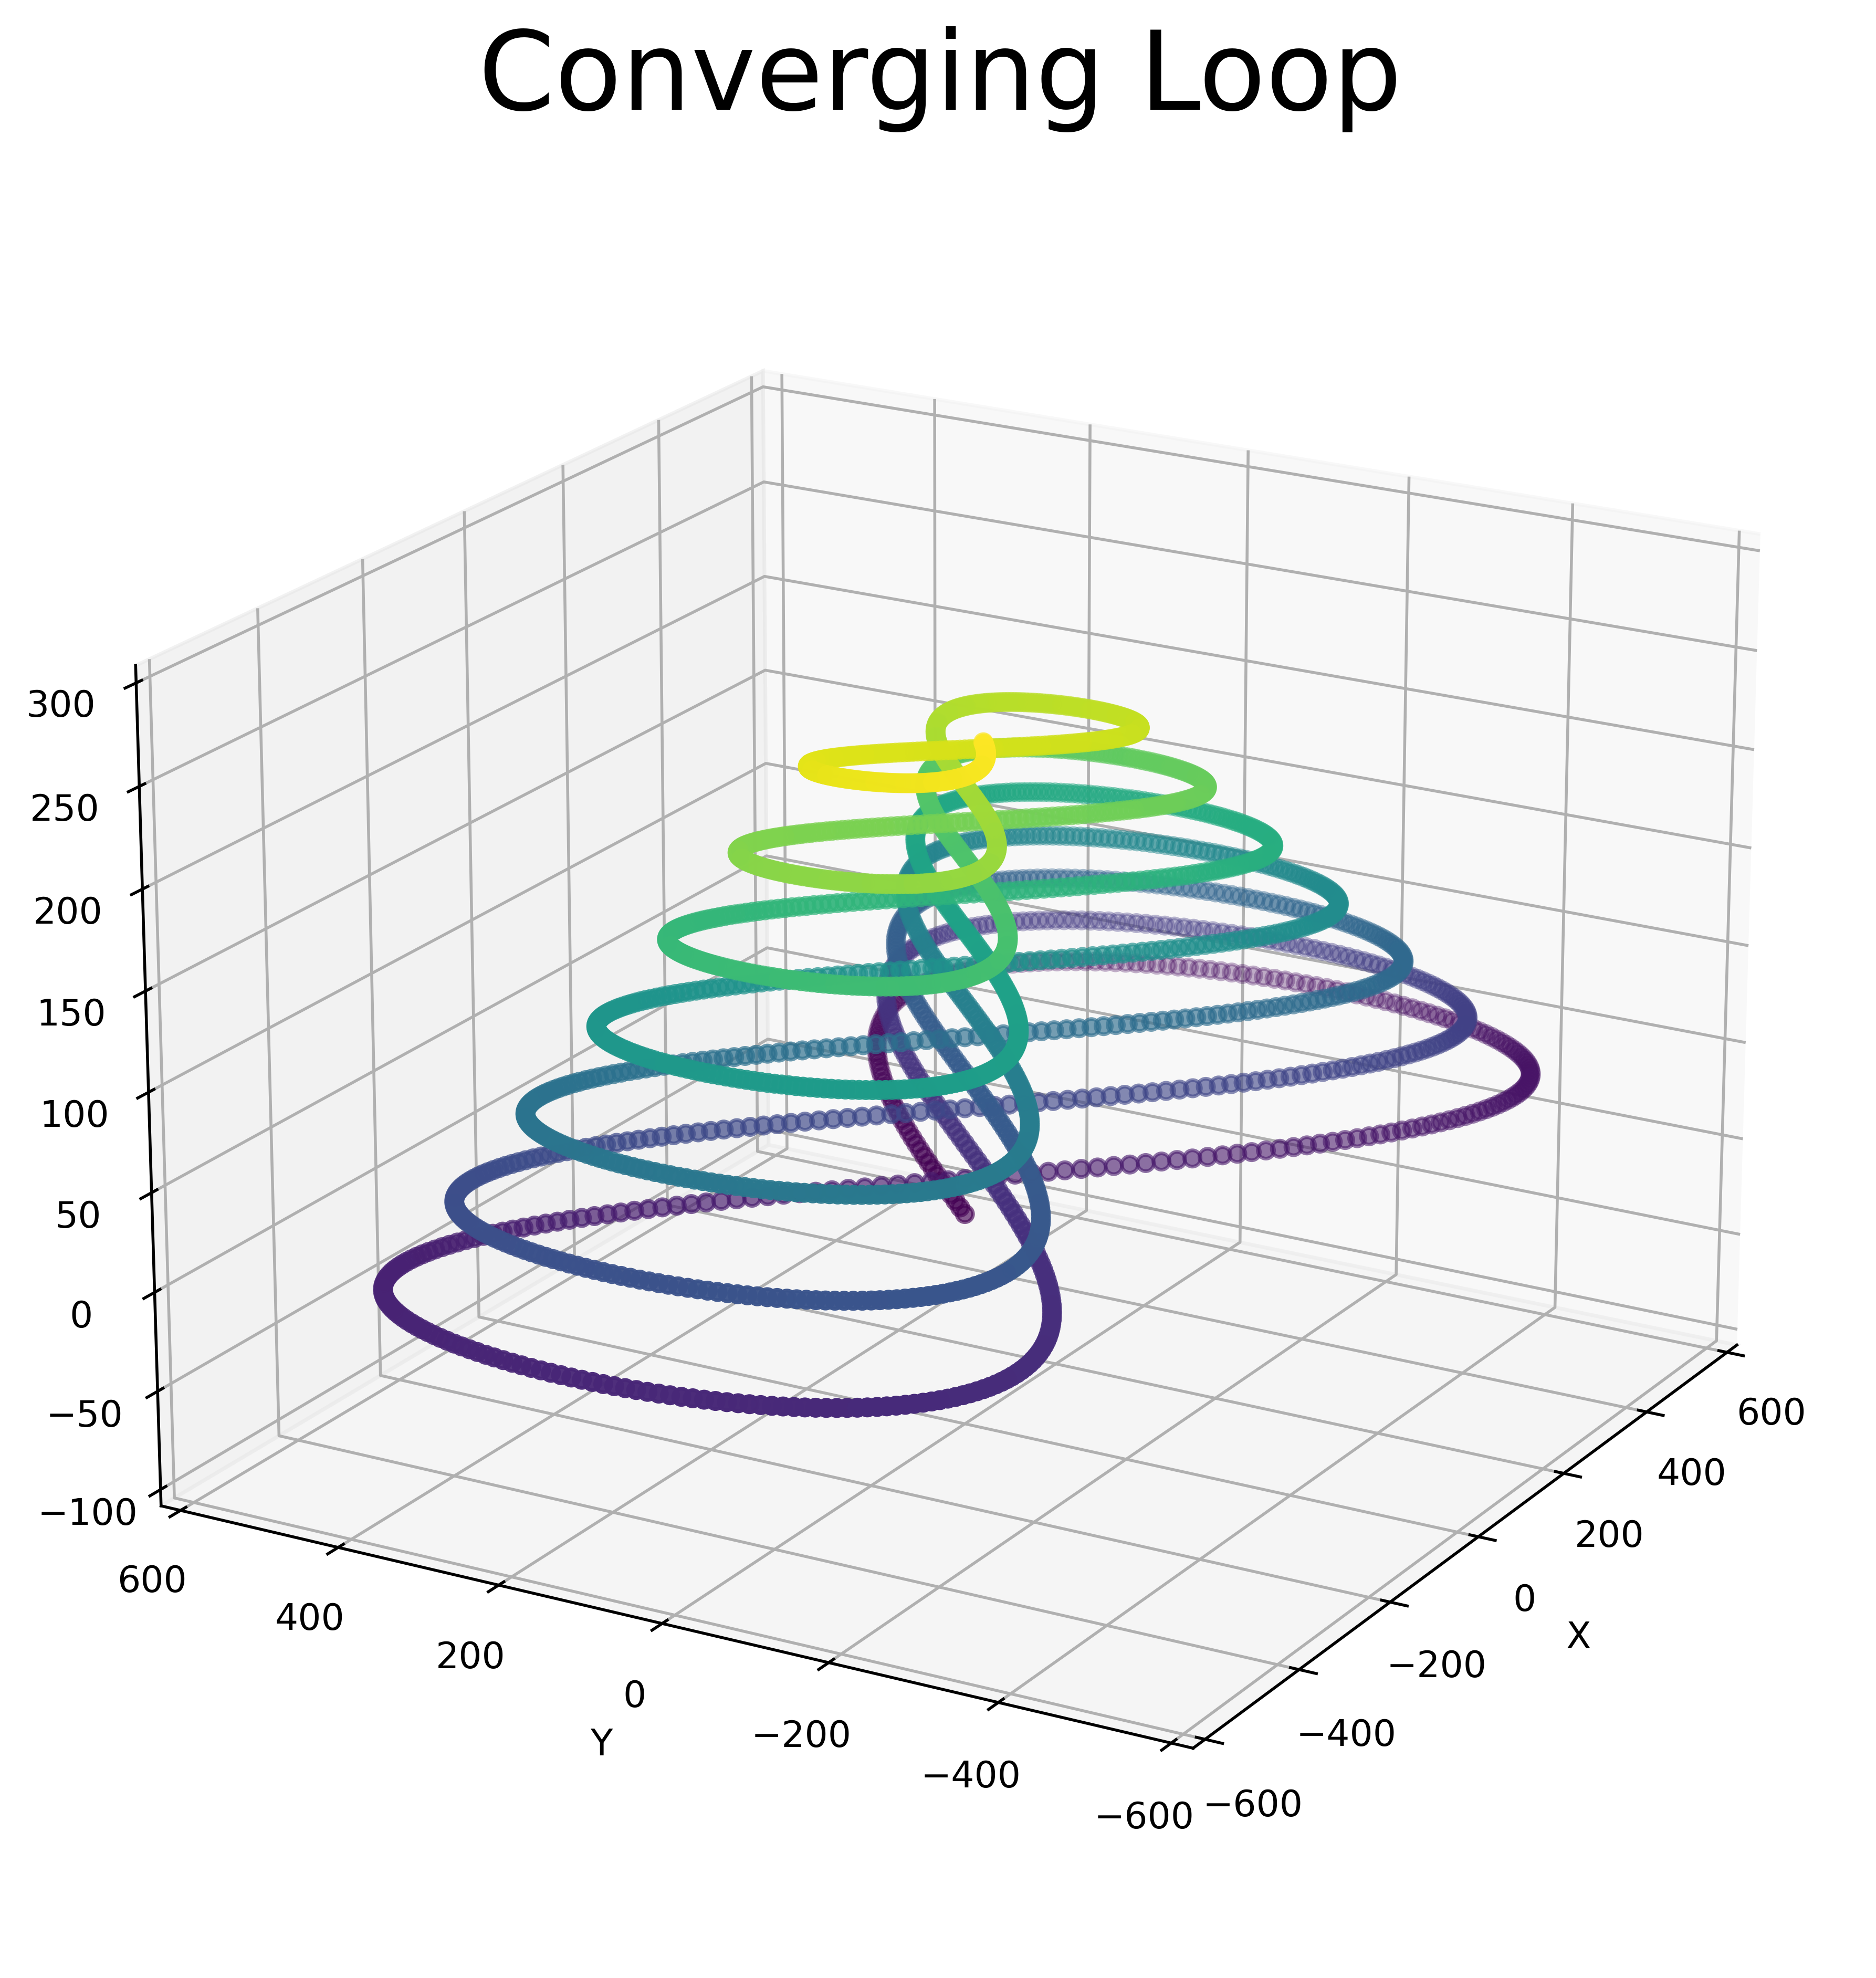
\includegraphics[width=0.5\textwidth]{figures/path2.png}}
	\caption{xxx}
	\label{xxxx}
\end{figure}
\begin{figure}[H]
	\centerline{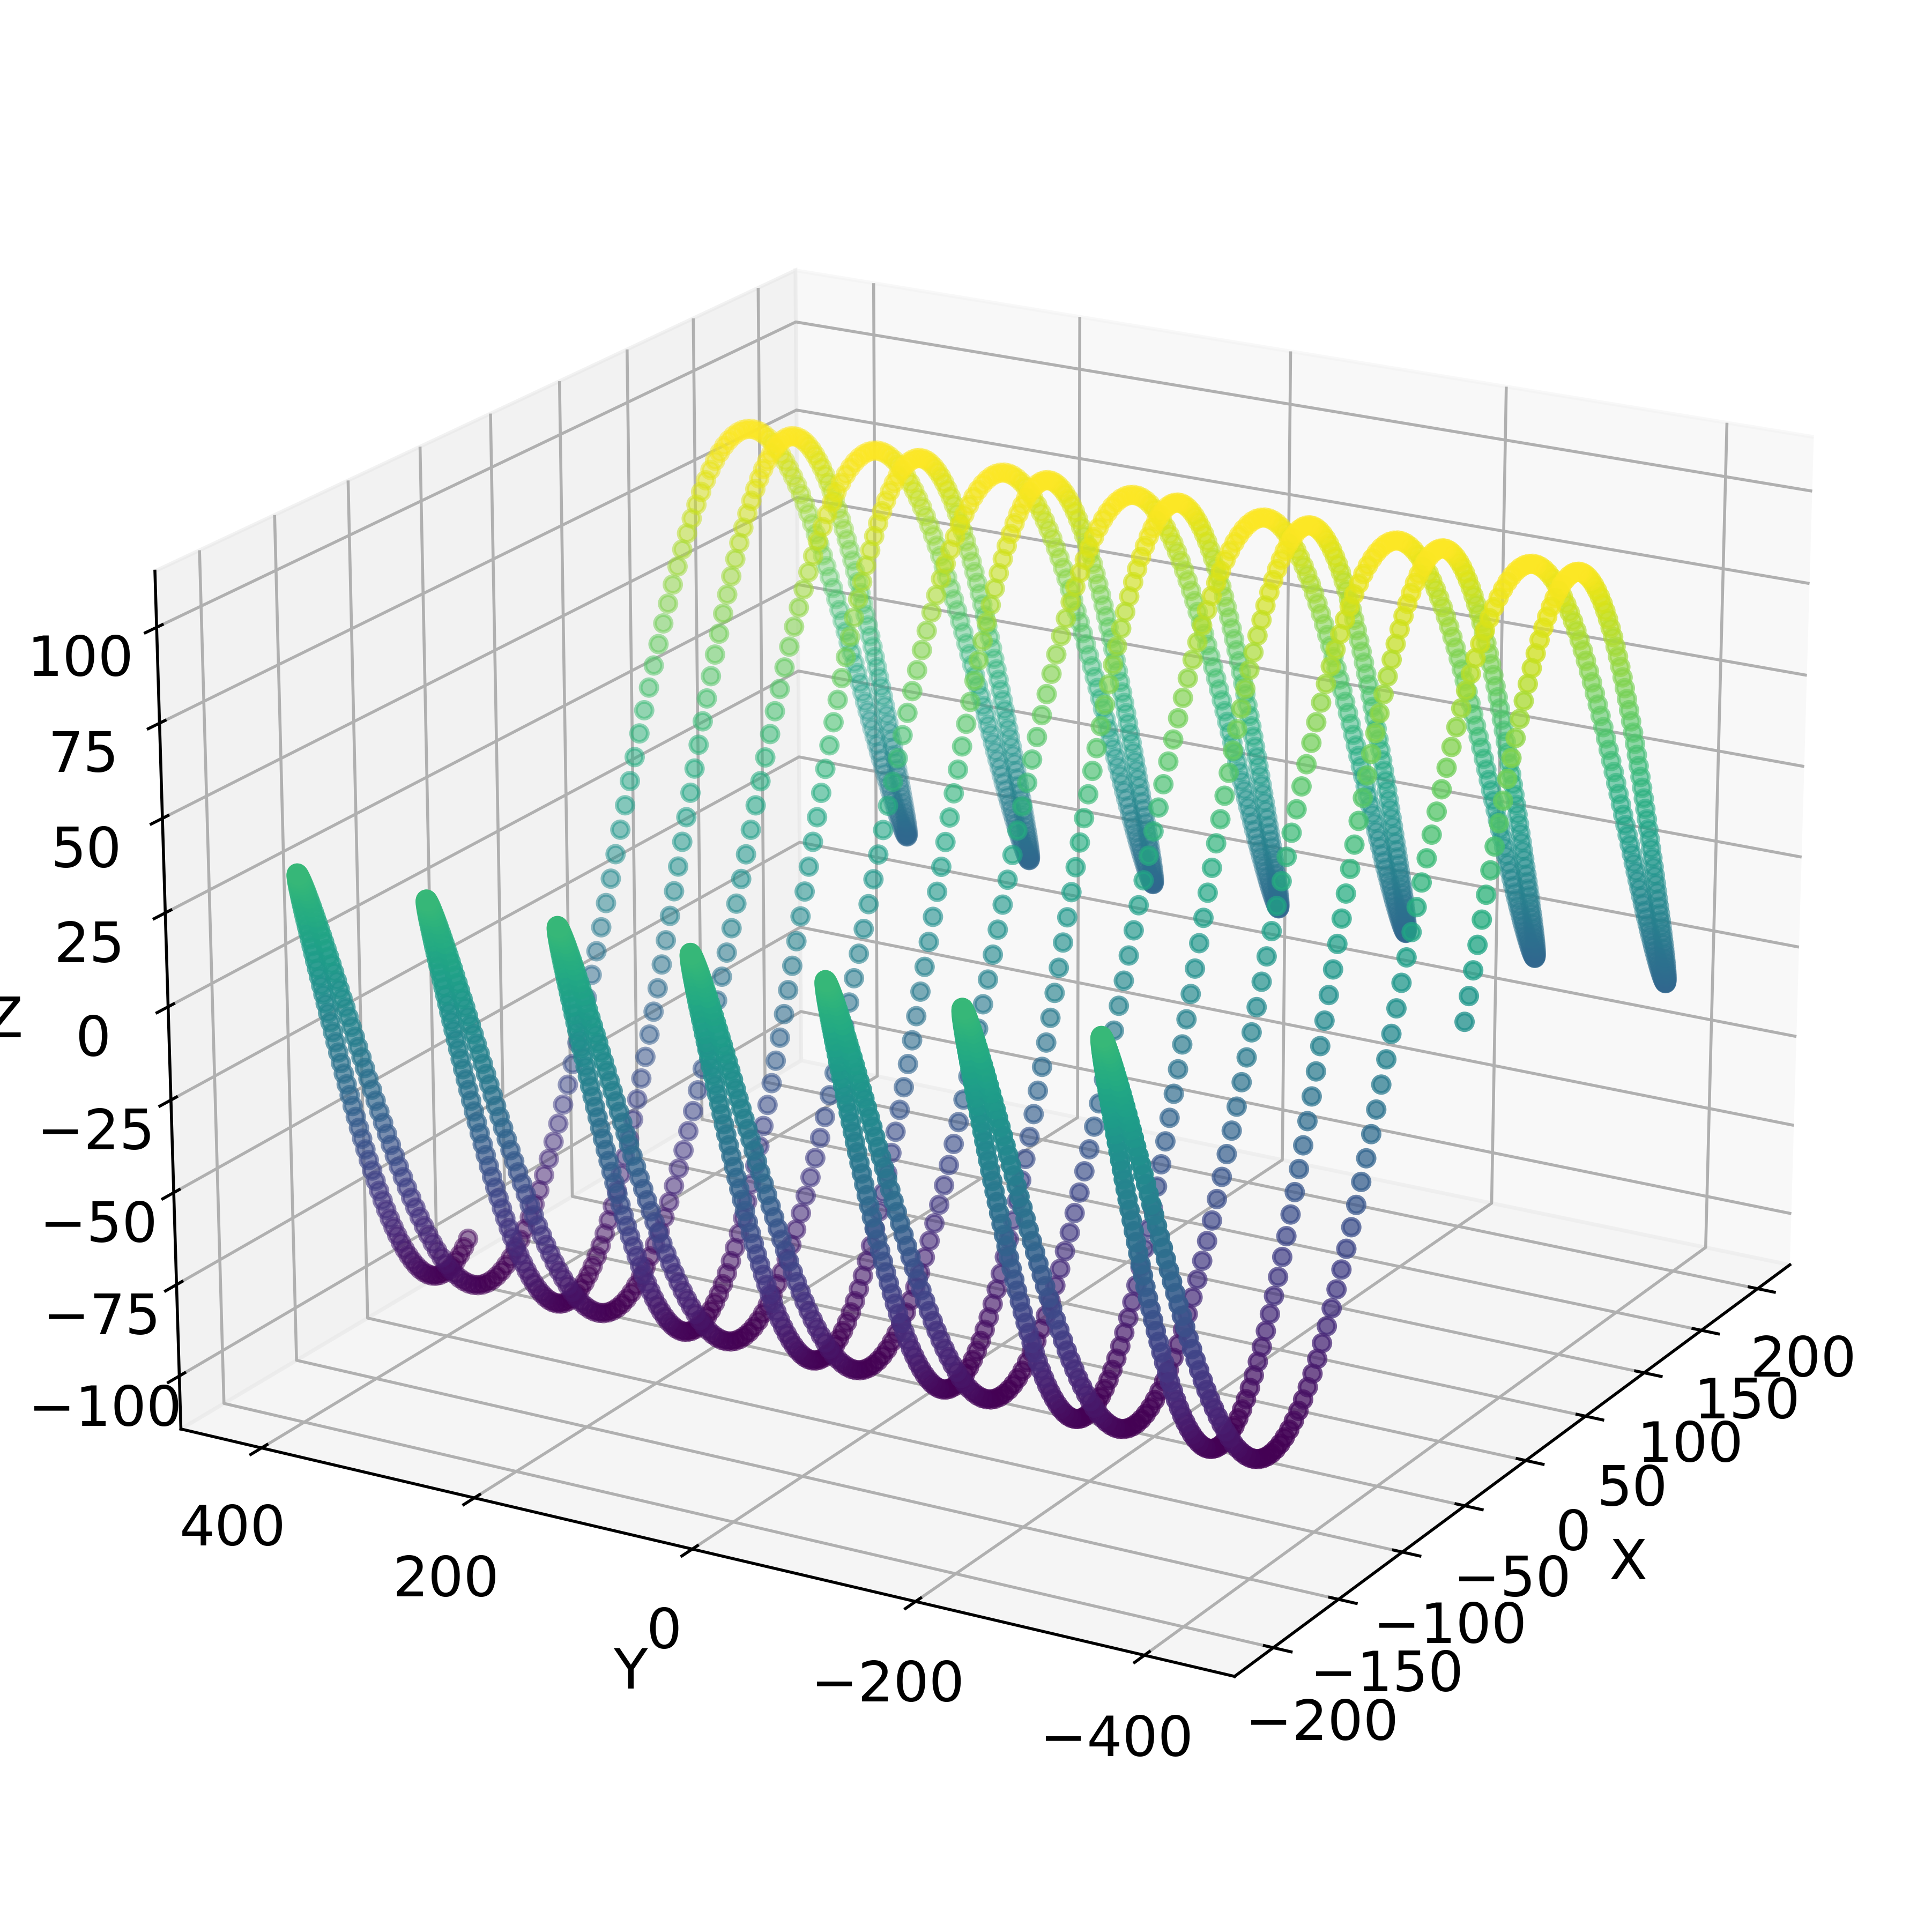
\includegraphics[width=0.5\textwidth]{figures/path3.png}}
	\caption{xxx}
	\label{xxxx}
\end{figure}

\subsection{Extracting process parameters}

\section{Testing and Validation}%

\section{Analysis and Discussion of the results}%


\subsection{Analysis}
\subsection{Discussion}%